\subsection{X-ray micro computed tomography}
\label{subsec:structure}
\Authors{Matthias Ruf (UoS)}
X-ray micro computed tomography ({\textmu}XRCT) is a non-destructive imaging technique and provides the possibility to examine the inner structure of an object by creating a digital 3D image of the same. It is based on the mathematical combination, called reconstruction, of several radiograms which were acquired from different directions. Thereby, a radiogram represents the respective measured intensity values $I(L)$ of the X-rays at position $x = L$ after travelling through the object and can be related to the unattenuated X-rays intensity $I_0$ before the object at position $x = 0$ by the Beer-Lambert law. Under the assumption of a monochromatic X-ray beam this can be written as 
\begin{align*}
I(L) = I_0 \exp\left(-\int_0^L \mu(x) \mathrm{d}x \right)
\end{align*}
for an inhomogeneous material with the unkown material depending attenuation coefficients $\mu(x)$ which are determined during the reconstruction process, cf. \cite{Carmignato2018}.

In Figure~\ref{fig:CTsystem} the self-made open and modular {\textmu}XRCT system at the Institute of Applied Mechanics - Chair of Continuum Mechanics of the University of Stuttgart, see \cite{Ruf2020} is depicted. 
\begin{figure*}[ht]
\centering
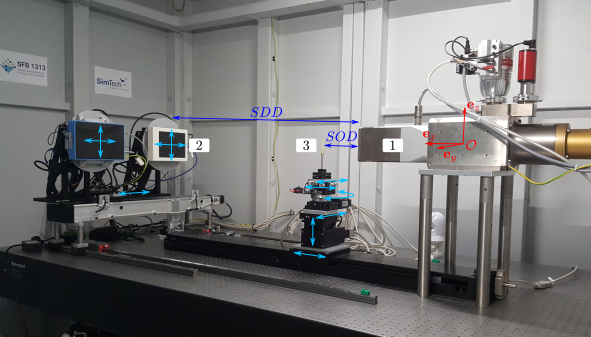
\includegraphics[width=1.0\textwidth]{figures/exp_2_2_xray_main.png}
\caption{Overview of the {\textmu}XRCT-system. The light blue arrows show the possible moving directions of the motorized stages.}
\label{fig:CTsystem}
\end{figure*}
It consists of the three main components: The X-ray source (1), the X-ray detector (2) and the sample positioning system including the rotation stage in between (3). Like most industrial CT-systems the specimen is rotated during the scan and the remaining parts are fixed. The employed X-ray tube provides a maximum power up to \SI{80}{\watt} and at the same time a focal spot size down to \SI{3}{\micro\meter} for moderate power levels. The acceleration voltage of the tube can be adjusted in the range of \SI{30}{\kilo\volt} to \SI{180}{\kilo\volt} and the flux from \SI{10}{\micro\ampere} to \SI{1000}{\micro\ampere}. It can be chosen between two indirect conversion flat panel detectors with different characteristics and resolutions of $1944 \times 1536$ and $2940 \times 2304$ pixels. Both produce gray value images with a pixel depth of \SI{14}{bit} and each is separately mounted on high accurate, motorized XY stages. The latter offers the possibility to compensate for bad detector pixels by taking several images from slightly different detector positions and subsequently stitching of the same to improve the final image quality.

The geometric magnification $M$ is given by the relation of the source detector distance $SDD$ to the source object distance $SOD$, $M = SOD/SDD$, and can be adjusted in a wide range. Depending on the sample material and the smallest feature size of interest, the specimen's diameter can be up to \SI{100}{\milli\meter}. The maximum achievable spatial resolution of the system is about \SI{50}{lp/mm} at \SI{10}{\%} of the modulation transfer function (MTF) which means a smallest feature size of \SI{10}{\micro\meter} that can be resolved. The corresponding field of view for this case is \SI{5.88}{\milli\meter} in width and \SI{4.60}{\milli\meter} in height. Therefore, the smallest expedient sample diameter is about \SI{5}{\milli\meter}. The open and modular concept of the CT-system provides a broad range also for unconventional investigations.

In Figure~\ref{fig:exampleCarraraMarble} a CT scan of a cylindrical Carrara marble core with a diameter of \SI{5}{\milli\meter} for a high resolution scan is shown exemplarily.
\begin{figure*}[ht]
	\centering
    \begin{subfigure}[c]{0.49\textwidth}
    \centering
	\label{fig:exampleCarraraMarble3D}
	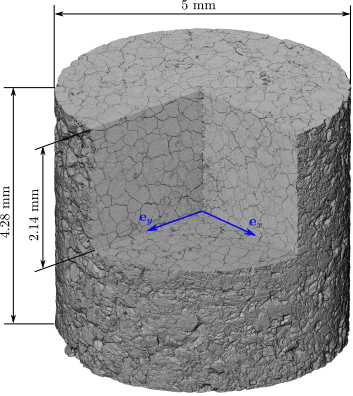
\includegraphics[width=0.9\textwidth]{figures/exp_2_2_scan_3d.png}
    \end{subfigure}
    \begin{subfigure}[c]{0.49\textwidth}
    \label{fig:exampleCarraraMarble2D}
	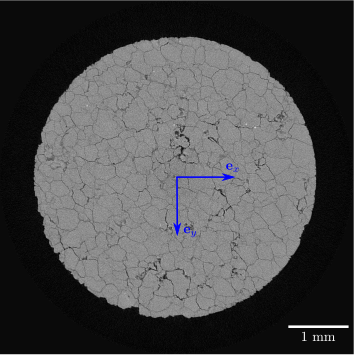
\includegraphics[width=0.9\textwidth]{figures/exp_2_2_scan_2d.png}
\end{subfigure}
\caption{CT scan of a Carrara marble core after thermal treatment.}
\label{fig:exampleCarraraMarble}
\end{figure*}

The visible micro-cracks along the grain boundaries were created by thermal treatment and are not present in the virgin state.  The geometric magnification was set to $M = 24.76$ which corresponds to the highest achievable spatial resolution and leads to a voxel size of \SI{2}{\micro\meter}. For additional details see \cite{Ruf2020}. Besides a qualitative assessment, the data sets offer the possibility of deriving several additional information by image processing. For instance, in geosciences the 3D pore characterization, the 3D grain analysis and the fracture analysis, cf. \cite{Cnudde2013}. 